\documentclass[12pt,a4paper]{article}
\usepackage{graphicx} % Required for inserting images
\usepackage{tikz}
\usepackage[left=2.00cm, right=1.00cm]{geometry}
\usepackage{xcolor} % before tikz or tkz-euclide if necessary
\usepackage{amsmath}
\usepackage{siunitx}
\usepackage{chemfig}
\usetikzlibrary{calc}
\begin{document}
\begin{center}
    \large\textbf{Arbeidsoppgaver om trykk:}
\end{center}
1.  Hvordan er temperaturskalaen Kelvin definert?\\\\
2.  Hva menes med det absolutte nullpunkt?\\\\
3. Hva sier den ideelle gasslov?\\\\
4.  Regn om til Kelvin:  $25 ^\circ C, 50^\circ C, -256^\circ C, 300^\circ C $\\\\
5. Regn om til celisus: 273,15K, 300K, 39K, 700K\\\\
6. En gass innestengt i beholder har et trykk på 3bar.  hvor stort blir trykket når vi halverer volumet og temperaturen er konstant? $V_1=3L$\\\\
7.  Vi har gitt følgende stempel med en gass som er innestengt.  Vi har et stempel som vi kan skyve inn og ut:\vspace{0.5cm}\\
\begin{center}
    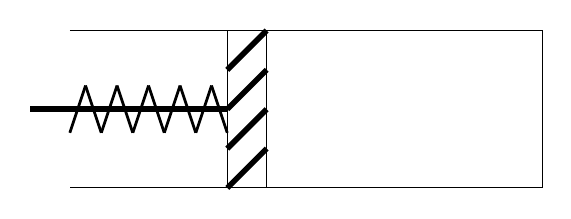
\begin{tikzpicture}
        %stempel med variabel
        \pgfmathsetmacro{\myLength}{4}
        \draw (2,2)--(8,2)--(8,0)--(2,0);
        \draw (\myLength,0)--(\myLength+0.5,0)--(\myLength+0.5,2)--(\myLength,2)--(\myLength,0);
        \draw [line width=2pt] (\myLength,0)--(\myLength+0.5,0.5);
        \draw [line width=2pt] (\myLength,0.5)--(\myLength+0.5,1);
        \draw [line width=2pt] (\myLength,1)--(\myLength+0.5,1.5);
        \draw [line width=2pt] (\myLength,1.5)--(\myLength+0.5,2);
        \draw [line width=2pt] (\myLength,1)--(\myLength-2.5,1);
        \draw [line width=1pt] (2,0.7)--(2.2,1.3);
        \draw [line width=1pt] (2.2,1.3)--(2.4,0.7);
        \draw [line width=1pt] (2.4,0.7)--(2.6,1.3);
        \draw [line width=1pt] (2.6,1.3)--(2.8,0.7);
        \draw [line width=1pt] (2.8,0.7)--(3.0,1.3);
        \draw [line width=1pt] (3.0,1.3)--(3.2,0.7);
        \draw [line width=1pt] (3.2,0.7)--(3.4,1.3);
        \draw [line width=1pt] (3.4,1.3)--(3.6,0.7);
        \draw [line width=1pt] (\myLength-0.4,0.7)--(\myLength-0.2,1.3);
        \draw [line width=1pt] (\myLength-0.2,1.3)--(\myLength,0.7);
    \end{tikzpicture}
\end{center}\vspace{1cm}
I starten er volumet $V_1=6L$ og trykket er lik $P_1=1,2bar$ .  Vi endrer volumet mens temperaturen er konstant slik at volumet blir $V_2=2L$.  Hva blir det nye trykket $P_2?$ \\\\
8.  Temperaturen til gasser er nå $T_1=25^\circ C$.  Vi øker temperaturen til 360K.  Hva blir det nye trykket $P_2$ om vi antar at volumet er konstant?\\

\noindent\textbf{Svar:}\\\\
1. Kelvinskalaen er definert ved at vi har en aller minste temperatur. Og den er er -273,15$^\circ C$.\\
2. Det absolutte nullpunkt er ved 0K. Da er temperaturen $-273,15^\circ C$
3. Den ideelle gasslov er:  $P\cdot V=n\cdot R\cdot T$\\
Der:\\
P=gassens trykk (Pa, $N/m^2$)\\
n=antall molekyl, eller mol.\\
R=gasskonstanten (8,314J/molK)\\
V=gassens volum ($m^3)$\\
T=temperatrun i K (kelvin)\\
4.  Regn om til Kelvin:  $25 ^\circ C, 50^\circ C, -256^\circ C, 300^\circ C $\\\\
$T(25^\circ)=25+273,15K=298,15K$\\
$T(50^\circ)=50+273,15K=323,15K$\\
$T(-2560^\circ)=-256+273,15K=17,15K$
$T(300^\circ)=300+273,15K=573,15K$\\\\
5. Regn om til celisus: 273,15K, 300K, 39K, 700K\\
$T(273,15K)=(273,15-273,15)^\circ  C=0^\circ C$\\
$T(300K)=(300-273,15)^\circ  C=26,85^\circ C$\\
$T(39K)=(39-273,15)^\circ  C=-234,15t^\circ C$\\
$T(700K)=(700-273,15)^\circ  C=426,85^\circ C$\\\\
6. En gass innestengt i beholder har et trykk på 3bar.  hvor stort blir trykket når vi halverer volumet og temperaturen er konstant? $V_1=3L$\\\\
Her må ha litt forklaring. Med utgangspunkt i ideell gasslov, så vil det for en ideell gass være sånn at:\\\\
$$\frac{P\cdot V}{T}=konstant$$\\\\
Vi tre spesialtilfeller, og det er når en av disse er konstant.  Da kan den "forkortes vekk" i formelen.  Det betyr at vi kan holde over den og så blir resten konstant.  I dette tilfellet så er T konstant. Vi får da:\\\\
$$P_1\cdot V_1=P_2\cdot V_2$$\\\\
Løst m.h.p. $P_2$:

$$P_2=\frac{P_1\cdot V_1}{V_2}=\frac{3bar\cdot 3L}{1,5L}=3bar\cdot 2=6bar$$
\end{document}